%2345678901234567890123456789012345678901234567890123456789012345678901
\chapter{Introduction to XML} % (fold)
\label{cha:introduction_to_xml}

	XML stands for eXtensible Markup Language. As the name implies,
	XML is a computer language for the tagging ---markup--- of
	data, or more precisely, an specification for writing
	particular markup languages. XML is Recommendation of the W3C
	since February 1998, and the latest XML 1.0 specification can
	be found at the W3C
	site\urlnote{http://www.w3.org/TR/REC-xml/}. For people not
	used to interpreting standard references, a solid reference
	guide to XML and related specifications is \emph{XML in a
	nutshell}~\cite{XML.Harold:2002dq}.
	
	The aim of this appendix is presenting astronomers, possibly
	with some development experience, with an introduction to XML,
	so that the VOTable appendix can be better understood.

	\section{Data markup} % (fold)
	\label{sec:data_markup}
		
		If we find the following set of data:
		
		\begin{adjustwidth}{0.1\columnwidth}{0.1\columnwidth}
			\begin{verbatim}
				Juan de Dios Santander Vela
				23/05/1972
				Ingeniero en Electrónica
				Instituto de Astrofísica de Andalucía
			\end{verbatim}
		\end{adjustwidth}
		
		\noindent we, as resourceful humans with lots of common
		sense, might think that the first line corresponds to the
		full name of a person, the second one is a date (most
		likely, a birth date), the third one is a degree (in
		Spanish), and the fourth one is an institution to which
		said person might belong.
		
		A non-ambiguous way to present the information above could
		be the following:
		
		\begin{adjustwidth}{0.1\columnwidth}{0.1\columnwidth}
			\begin{verbatim}
				NAME:          Juan de Dios Santander Vela
				BIRTHDATE:     23/05/1972
				DEGREE(es_ES): Ingeniero en Electrónica
				INSTITUTION:   Instituto de Astrofísica de Andalucía
			\end{verbatim}
		\end{adjustwidth}
		
		That, for instance, is the kind of convention used in FITS
		header cards~\cite{1981A&AS...44..363W}: using keywords for
		particular pieces of data, and putting the data after said
		keywords.
		
		However, that system brings its own share of problems. For
		instance, what kind of keywords must be admitted? How many
		degrees can a person have, or how many institutions can
		that person belong to? If we wish to provide the same
		information for a large number of people, how does a
		computer recognise the end of each record?
		
	% section data_markup (end)
	
	\section{XML markup} % (fold)
	\label{sec:xml_markup}
		
		In XML, those problems are solved by following these rules:

		\begin{description}
			\item[Tags enclose marked up data] A piece of data is
			marked up by enclosing it between \xmlopen{TAG} and
			\xmlclose{TAG}. For instance, a person's name would be
			a string enclosed between \xmlopen{NAME} and
			\xmlclose{NAME}, as in \xmlenclose{NAME}{Juan de Dios
			Santander Vela}.
			
			\item[Tags are case sensitive] In an XML document, all
			of the following are different tags: \xmlopen{NAME},
			\xmlopen{name}, \xmlopen{Name}. However, it is strongly
			recommended not to use tags which only differ in their
			capitalisation.
			
			\item[At the root of an XML document, one and only one
			tag exists] In XML documents,
			everything is inside a tag. If more tags need to be
			specified, they must be enclosed in a higher hierarchy
			tag. With this in mind,
			
			\xmlenclose{NAME}{Juan de Dios Santander Vela}\\
			\xmlenclose{BIRTHDATE}{23/05/1972}
			
			\noindent is not a valid XML document, but
			
			\xmlenclose{PERSON}{\\ \xmlenclose{NAME}{Juan de Dios
			Santander Vela}\\ \xmlenclose{BIRTHDATE}{23/05/1972}\\
			}
			
			\noindent is.
			
			\item[All tags reside completely within other tags]
			This condition means that for closing a tag, all other
			tags that might have opened inside must be closed. That
			is, \xmlopen{strong}\xmlopen{em}\texttt{This is a text
			marked up with bold and italics}
			\xmlclose{strong}\xmlclose{em} is not valid XML, as the
			\xmltag{em} opens after the \xmltag{strong}, but the
			\xmltag{em} is still open when trying to close
			\xmlopen{strong}.
			
			The last two conditions are also commonly stated as:
			\emph{XML documents must be well-formed}. That is,
			\emph{well-formedness} is the property of an XML
			document of having just a single root element, and
			having elements completely enclosed within other
			elements.
		\end{description}
		
		Additionally, XML tags can hold extra attributes. For
		instance, the \xmltag{DEGREE} can have an
		\xmlattr{language} which specifies the language and country
		in which the degree was awarded, i.e.,
		\xmlencloseattr{DEGREE}{lang=`es\_ES'}{Ingeniero en
		Electrónica}.
		
		 With those rules, the information above might be written
		in XML as:
		
		\begin{adjustwidth}{0.1\columnwidth}{0.1\columnwidth}
			\noindent\xmlenclose{PERSONS}{\\
				\xmlenclose{PERSON}{\\
					\xmlenclose{NAME}
						{Juan de Dios Santander Vela}\\
					\xmlenclose{BIRTHDATE}{23/05/1972}\\
					\xmlencloseattr{DEGREE}{lang="es\_ES"}
					{Ingeniero en Electrónica}\\
					\xmlenclose{INSTITUTION}
					{Instituto de Astrofísica de\\Andalucía\\}\\
				}\\
			}
		\end{adjustwidth}
		
		An additional \xmltag{PERSONS} has been included so that
		several \xmlopen{PERSON} records could be found in the same
		XML document.
	% section xml_markup (end)
	
	\section{XML validation} % (fold)
	\label{sec:xml_validation}
		
		In the example above, we have devised an XML-based markup
		whose root element is the \xmltag{PERSONS}, which can hold
		inside one or more \xmltags{PERSON}, each one containing
		\xmlopen{NAME}, \xmlopen{BIRTHDATE}, \xmlopen{DEGREE} and
		\xmltags{INSTITUTION}.
		
		 However, as there is been no specification of the
		language, how can a computer make sure that the
		\xmltag{INSTITUTION} belongs in the \xmltag{PERSON}? What
		can be put inside a \xmltag{BIRTHDATE}?
		
		 In other words, how can we specify a particular XML markup
		language so that computers can validate particular XML
		document (instances) against that specification?
		
		 As originally XML was a subset of an existing markup
		language called Standard Generalized Markup Language
		(SGML), XML documents used the SGML mechanism for markup
		specification, called Document Type Definition (DTD). DTDs
		specify \texttt{ELEMENT}s, which are the particular tags
		which can appear in an XML document referencing the DTD,
		and \texttt{ATTLIST}s (attribute lists), which are the sets
		of attributes that can modify a particular tag. The
		\texttt{ELEMENT} declarations' syntax also allows for
		specifying which tags can occur, and how many times, inside
		others.
		
		 A DTD specifying the \texttt{ELEMENT}s and
		\texttt{ATTLIST} for the example above would be:
		
		\begin{adjustwidth}{0.1\columnwidth}{0.1\columnwidth}
			\dtdelement{PERSONS (PERSON*)}\\
			\dtdelement{PERSON
			(NAME,BIRTHDATE?,DEGREE*,INSTITUTION*)}\\
			\dtdelement{NAME (\#PCDATA)}\\
			\dtdelement{BIRTHDATE (\#PCDATA)}\\
			\dtdelement{DEGREE (\#PCDATA)}\\
			\dtdelement{INSTITUTION (\#PCDATA)}\\
			\dtdattlist{DEGREE lang CDATA \#REQUIRED}
		\end{adjustwidth}
		
		The rules for DTDs are:
		
		\begin{itemize}
			\item \dtdelement{tag (tagcontents)} indicates that
			\xmltags{tag} are allowed, with \texttt{tagcontents}
			inside.
			
			 \item \texttt{tagcontents} is either a single tag, a
			list of tags separated by commas (\texttt{,},
			indicating several tags which may appear in sequence),
			a list of tags separated by the vertical bar
			(\texttt{|}, indicating alternative tags which might
			appear), the keyword \texttt{ANY} (indicating that any
			tag can occur inside), or the keyword \texttt{EMPTY}
			(indicating that the \xmltag{tag} must have no content,
			and can be used as \xmlself{tag}. All the tags
			appearing inside a \texttt{tagcontents} must have a
			corresponding \dtdelement{tag} entry.
			
			 \item The number of times a tag specified in
			\texttt{tagcontents} can appear depends on certain
			modifier characters after the tag. The asterisk
			(\texttt{*}) indicates that a tag can appear any number
			of times, including none at all. The question mark
			(\texttt{?}) indicates that the tag is optional, and
			can appear once or none at all. A plus sign
			(\texttt{+}) indicates that the tag must appear at
			least once, but can appear many more times. If no
			symbol is specified, the tag appears just one time.
			
			 \item \dtdattlist{tag attrName attrType defaultValue}
			specifies that the \xmltag{tag} can have an attribute
			\texttt{attrName}. \texttt{attrType} is one of:
			\texttt{CDATA} (for strings); \texttt{(a|b|...|n)} (for
			an attribute which can be any one of \texttt{a} to
			\texttt{n}); \texttt{ID} (for a unique identifier);
			\texttt{IDREF} (for a reference to an \texttt{ID} of a
			different element); \texttt{IDREFS} (for a
			space-separated list of \texttt{ID}s to different
			elements); and additional specifiers for entities and
			entity lists (entities are symbols representing
			particular characters or strings, such as
			\texttt{\&amp;} representing the ampersand
			(\texttt{\&})), shared controlled vocabularies (for
			attributes with the same list of possible values). And
			\texttt{defaultValue} is either \texttt{``value''},
			indicating the \texttt{attrName} can be set to any
			value, but if not \texttt{value} is applied by default;
			\texttt{\#IMPLIED} for attributes which do not need to
			be set, and for which no default value is assumed;
			\texttt{\#REQUIRED} for attributes which must be set
			with any value; or \texttt{\#FIXED ``value''} for
			attributes which must be set exactly to \texttt{value}.
		\end{itemize}
		
		If we take into account the rules above, our DTD states
		that:
		
		\begin{enumerate}
			\item The \xmltag{PERSONS} contains any number of
			\xmltags{PERSON}, but \xmltags{PERSON} alone. The root
			\xmltag{PERSONS} must exist. (\texttt{tagname*} denotes
			any number, including none, of \xmltags{tagname}, while
			\texttt{tagname} alone means one and only one
			\xmltag{tagname} appearance.)
			
			 \item The \xmltag{PERSON} contains, in order, one
			\xmltag{NAME}, and optionally a \xmlopen{BIRTHDATE},
			any number of \xmltags{DEGREE}, and any number of
			\xmltags{INSTITUTION}.
			
			 \item Inside the \xmlopen{NAME}, \xmlopen{BIRTHDATE},
			\xmlopen{DEGREE} and \xmltags{INSTITUTION} (that is,
			enclosed between \xmlopen{tag} and \xmlclose{tag}), the
			content can be any string (\texttt{\#PCDATA}).
			
			 \item The \xmltag{DEGREE} has a required attribute,
			\texttt{lang}, which is a string (\texttt{CDATA}).
		\end{enumerate}
		
		A valid XML document is one which is not only well-formed,
		but which also follows the prescriptions of the DTD
		regarding allowed tags, allowed tag content and cardinality
		restrictions (the number of times a tag can appear), as
		well as restrictions on allowed attributes.
		
	% section xml_validation (end)
	
	\section{XML semantics} % (fold)
	\label{sec:xml_semantics}
		
		To this moment, we have considered the validity of XML
		documents with regard to certain automatic checks to be
		performed regarding the contents of several tasks. But what
		about the semantics of XML documents?
		
		 Semantics, regarding data markup, is precisely the
		relationship between a marked-up datum and an existing
		object (real or virtual) for which a particular property is
		being stated. The relationship must be one-to-one from the
		data markup and the property of interest.
		
		 We can see that for particular XML languages, specified by
		a DTD, the \dtdelement{elementName} tags introduce a
		hierarchy of elements for which data (or metadata) have to
		be provided, whereas \dtdattlist{attribName} indicate
		additional metadata for elements.
		
		 That way, DTDs establish a data model for describing data
		in a particular scope. In the case of astronomical data
		interchange, XML documents are called VOTables. Initially,
		VOTables were XML documents conforming to the VOTable DTD
		(see section~\ref{sec:votable_dtd} in
		appendix~\ref{cha:votable_format_definition}).
		
		 However, DTDs do not impose strong restrictions on
		particular datum a tag can hold, other than enumerating
		\emph{a priori} all possible values. However, if a datum
		must be an URI (as in a \texttt{href} attribute within a
		\xmltag{LINK}), there are practical restrictions on what
		can constitute a valid URI and what not, but they cannot be
		described in a DTD. Thats what the XML Schema language is
		for: defining data types which carry their own semantics,
		and expressing tighter restrictions which help in defining
		such semantics.
	% section xml_semantics (end)
	
	\section{The XML Schema language} % (fold)
	\label{sec:xml_schema}
		
		The XML Schema language is a set of XML keywords which can
		be used to express everything a DTD can express, in terms
		of data modelling, but with many additional features:
		
		\begin{description}
			\item[Better defined restrictions] DTDs can only
			express the restrictions on data exposed on
			section~\ref{sec:xml_validation}. However, many times
			additional restrictions must be imposed on data, such
			as ensuring certain contents conforms to given regular
			expresions.
			
			 \item[Data types] In computer languages, data types
			are very much akin to physical units, in the sense that
			variables of a particular data type can only hold, be
			compared to, or added to values of that same (or
			compatible) data types. XML Schema can be used to
			create data types, and then assign those data types
			(which by themselves impose restrictions on data) to
			elements (or attributes) which must conform to those
			data types. This aids both in better reuse of datatypes
			across the schema, and a much more modular design.
			
			 \item[Namespaces] Namespaces are an XML feature quite
			related to semantics and modularity. Namespaces allow
			the usage of tags from different XML Schemata in the
			same XML document, so that the particular meaning for a
			tag within a given schema is preserved, together with
			the restrictions and relationships set by each schema.
			
			 \item[XML Schema is expressed in XML] This means that
			the file expressing the restrictions/data types for XML
			documents of the type conforming to said schema is, by
			itself, an XML document, so that XML tools can be used
			for verifying the schema validity, or for using the
			XQuery language to find usages of a data type, or the
			XSLT language for creating a DTD, or any other kind of
			representation, from the Schema document. However, that
			also means that XML Schemas tend to be much more
			verbose than DTDs for the same file type.
		\end{description}
		
		We will not enter in detail into the XML Schema language,
		as it is ouside the scope of this appendix. The official
		W3C specification can be found at
		\url{http://www.w3.org/TR/xmlschema-1/}.
		
	% section xml_schema (end)
	
	\invisiblenote{
	\section{Related XML technologies} % (fold)
	\label{sec:related_xml_technologies}
		
		However, we will provide astronomical developers
		with some pointers to the main XML related technologies
		to be found when processing XML documents.
		
		\subsection{Document Object Model (DOM)} % (fold)
		\label{sub:dom_document_object_model}
			For XML documents whose whole content is to be
			processed programmatically, it can be useful to create
			a computing object based on XML contents. For instance,
			from the XML documents shown on
			section~\ref{sec:xml_markup}, the following class tree
			(with branches shown by the dot (\texttt{.}) operator)
			would be created, as per the DTD and the document
			content:
			
			\begin{itemize}
				\item \texttt{PERSONS[]}, as an array of
				\texttt{PERSON} objects;
				
				 \item \texttt{PERSONS[i].PERSON} is an object
				containing the i-th \texttt{PERSON} data);
				
				 \item \texttt{PERSONS[i].PERSON.NAME} is a String
				object, holding the name of the i-th person;
				
				 \item \texttt{PERSONS[i].PERSON.BIRTHDATE} is a
				String object, holding the birthdate of the i-th
				person;
				
				 \item \texttt{PERSONS[i].PERSON.DEGREE[]} is an
				array of \texttt{DEGREE} objects, where the j-th
				degree of the i-th person is held in
				\texttt{PERSONS[i].PERSON.DEGREE[j]};
				
				 \item \texttt{PERSONS[i].PERSON.INSTITUTION[]} is
				an array of \texttt{INSTITUTION} objects, with
				\texttt{PERSONS[i].PERSON.INSTITUTION[j]} holding
				the j-th institution to which the i-th person
				belongs to.
			\end{itemize}
			
			The corresponding tree is shown in
			figure~\ref{fig:fig_persons}.

			\begin{figure}[tbp]
				\centering
					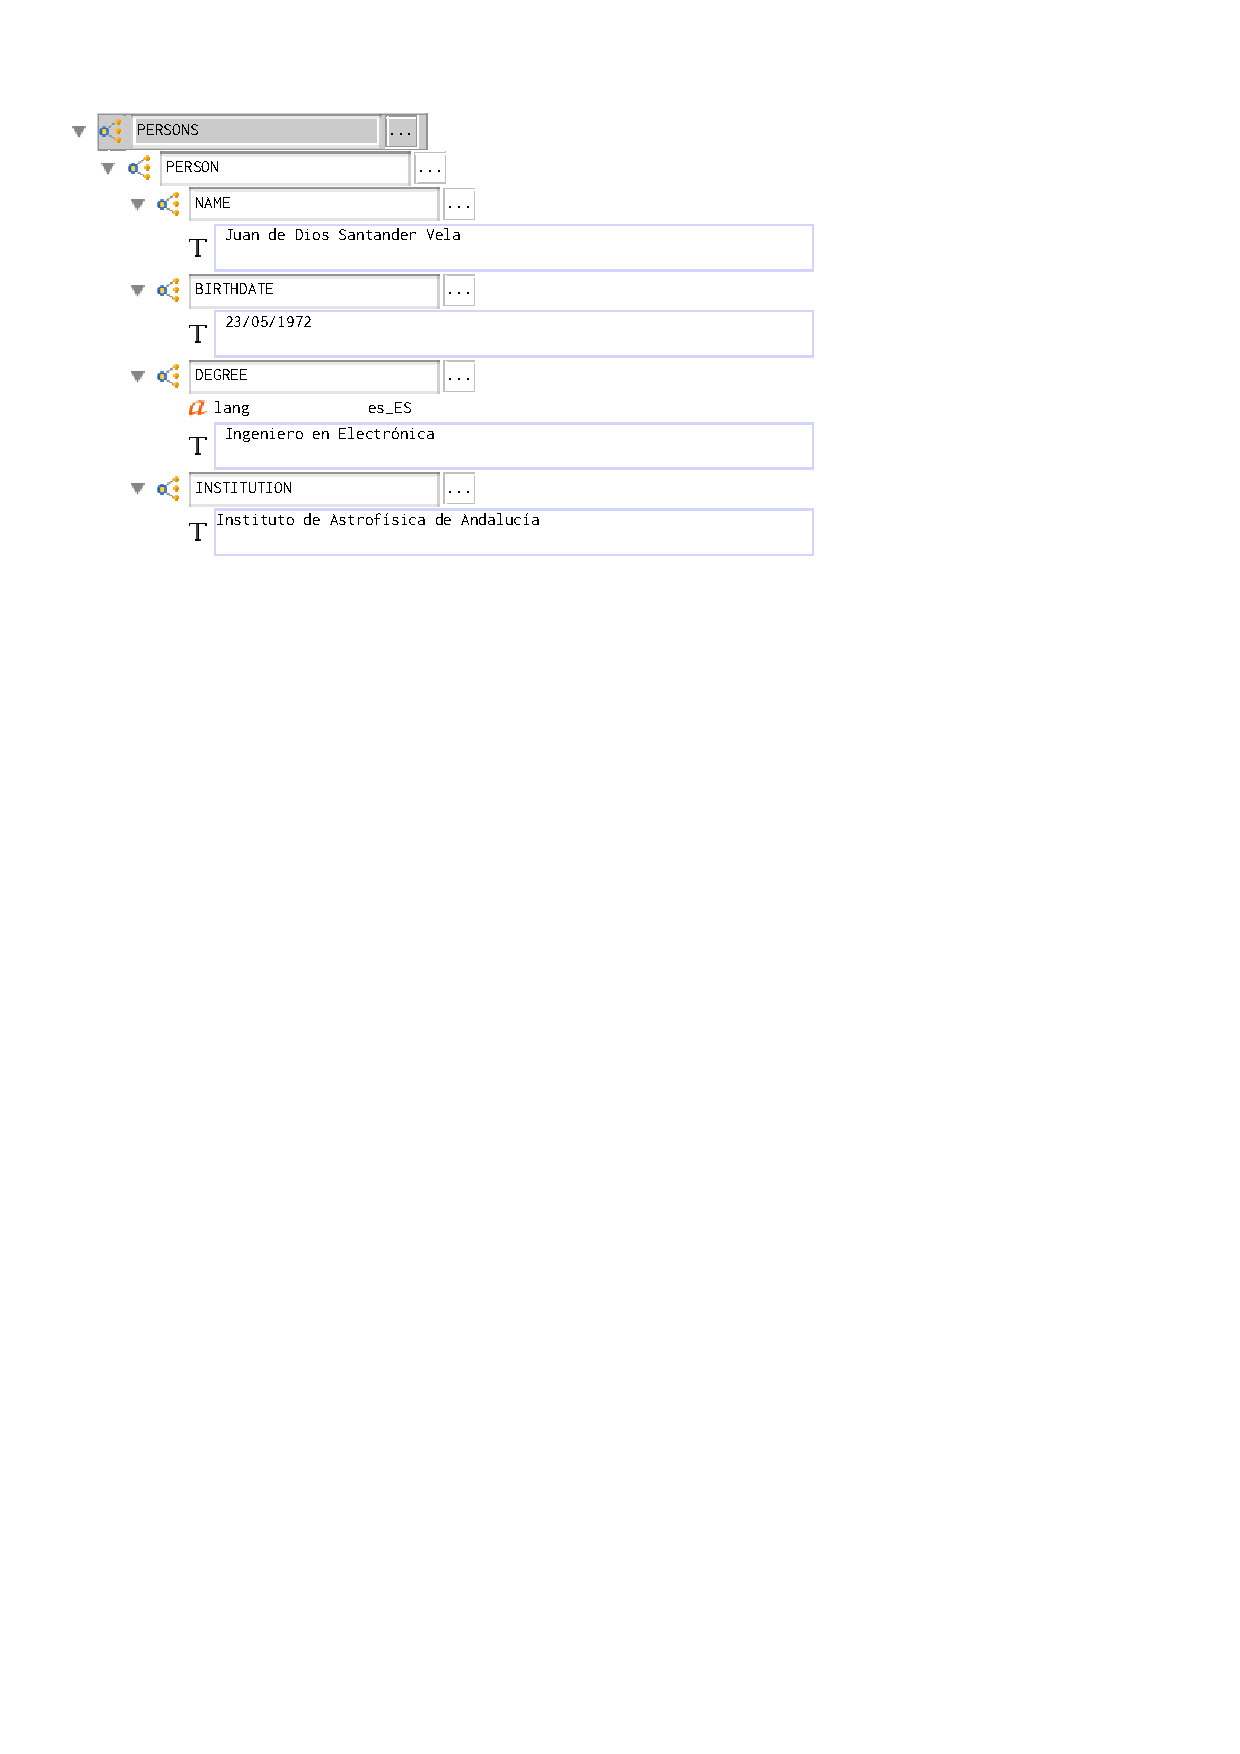
\includegraphics[width=\columnwidth]
					{fig/persons.pdf}
				\caption[Vista en árbol de un archivo XML]{
					Vista en árbol correspondiente al archivo XML
					anteriormente presentado. Se puede ver cómo de
					\texttt{PERSONS} cuelgan varios \texttt{PERSON}
					(en este caso sólo uno), de cada
					\texttt{PERSON} pueden colgar \texttt{NAME},
					\texttt{BIRTHDATE}, \texttt{DEGREE} e
					\texttt{INSTITUTION}. Se puede continuar el
					árbol incluyendo el contenido de cada etiqueta,
					y los posibles atributos que contenga.
			}
				\label{fig:fig_persons}
			\end{figure}
			
			In the DTD we defined a \texttt{lang} attribute to the 
			
			\todo{Finish attribute}
			
		% subsection dom_document_object_model (end)
		
		\subsection{XPath} % (fold)
		\label{sub:xpath}
			\todo{Finish XPath}
		% subsection xpath (end)
		
		\subsection{XQuery} % (fold)
		\label{sub:xquery}
			\todo{Finish XQuery}
		% subsection xquery (end)
		
		\subsection{XSLT} % (fold)
		\label{sub:xslt}
			\todo{Finish XSLT}
		% subsection xslt (end)
		
	% section related_xml_technologies (end)
	
	\section{XML libraries} % (fold)
	\label{sec:xml_libraries}
		There are many different XML manipulation, creation, and
		validation libraries, for many different languages. We
		point out the main contenders, classified by language.
		
		\subsection{C/C++/compiled libraries} % (fold)
		\label{sub:c_cpp_compiled}
			\begin{description}
				\item[libxml] libxml was born originally as the XML
				library for the Gnome X11 window manager project,
				but it can be used and found elsewhere (for
				instance, in Mac OS X it is found installed by
				default). Provides tools for parsing and validating
				XML documents, as well as item selectors such as
				XPath or XPointer, XML inclusions, et cetera. It
				can be found at \url{http://xmlsoft.org/}.
				
				 \item[libxslt] lbxml is the XSLT transformations
				library for It can be found at
				\url{http://xmlsoft.org/XSLT/}.
				
				 \item[SAX] stands for \emph{Simple API for XML}.
				It was originally developed for Java, but bindings
				for other languages exist for it. SAX is an
				event-based API, where finding tags and/or data in
				the XML document trigger some functions in the
				parsing application. Compare with tree-based APIs,
				which give the application full access to the
				document, but which are unsuitable for very large
				documents.
			\end{description}
			
		% subsection c_cpp_compiled (end)
	% section xml_libraries (end)
	}

% chapter introduction_to_xml (end)